\documentclass{article}
\usepackage[top=1in, bottom=1.25in, left=1in, right=1in]{geometry}
\usepackage{hyperref}
\usepackage{graphicx}
\usepackage{csquotes}
\usepackage{amsmath}
\usepackage{setspace}
\usepackage{float}
\usepackage{caption}
\usepackage[font=small, labelfont=bf]{subcaption}
\usepackage{lscape} %landscape
\renewcommand{\familydefault}{\sfdefault} %change font

\begin{document}
\doublespacing
\setlength{\parindent}{0pt}
\section{Purpose of this research}

In this study, we plan to find dissimilarities between normal cells and cancerous cells,
through investigating HiC contact maps. 
We suspect that there are systematic differences between how chromosomes are structured
between normal cells and cancerous cells.
we 
Ideally, it is desirable to compare 3D structures of 
cell in order to make such comparisons.
However, the main challenge that we face is that 
3D structure of a cell is not readily available. Based on
\cite{adhikari2016chromosome3d}, fluorescence in situ hybridizaiton
(FISH) is used for investigating 3D configuration of chromosomes.
However, this method can only be used locally and cannot map
the whole structure of the chromosomes.
In orther to find dissimilarities in the 3D structure of 
chromosomes, we used HiC dataset.
The HiC method, which was developed by \cite{lieberman2009comprehensive}, captures interactions between 
chromosomal fragments in kilobase resolution. Based on HiC data, an
\textit{interaction frequency (IF) } matrix can be developed between \textit{loci} at a desired resolution.
A cell $IF_{ij}$ in an interaction frequency matrix captures the number of interaction detected
in HiC dataset between locus $i$ and locus $j$ in the genome.
An interaction matrix can be used to develop both inter- and intra-chromosomal interaction matrices.
We believe differences in interaction matrices can be found between normal cells and cancerous ones.

\section{Genetics and Genomics}
\textbf{What is genetics?}
studies heredity. Offspring resembles its parents becasue they
inherit their \textit{genes}.\\
\textbf{Gene}: Sets of instructions that determine the traits of an organism.
A sequence of DNA. A DNA thread builds chromosomes.
Each organism has a unique number of chromosomes:
Humans: 46 chromosomes. You get 23 from your mother and 23 from your
father.\\
\textbf{Homologous chromosomes}: A set of two chromosomes consisting of genes
that correspond to the same traits, one coming from mother and the 
other coming from father. These corresponding genes are called
\textit{alleles}. Alleles are either \textit{dominant} or \textit{
    recessive}.\\
\textbf{Phenotype vs. Genotype}: Phenotype is a visible physical trait that
is caused partially by genes and partially environmental.
These traits include eye of hair color, height etc.
\textit{genotype} is the gense that correspond to a particular
phenotype. 
Their presence is necessary but not enough for the 
existence of phenotype.

\textbf{Homozygous vs. Heterozygous alleles}:
There are 3 combinations of genotypes:
tt, tT (or Tt) and TT. 
If the two alleles are the same
then the person is Homozygous (dominant or recessive)
in the corresponding
trait. Otherwise, the person is Heterozygous in that trait.

\textbf{Nucleotide}:  The monomer units that comprise DNAs. There
 are 4 types of nucleotides: (C, G, A, and T)

\textbf{DNA}: Macro-molecules that provide recipes for creating 
proteins.

\textbf{Gene Expression}:
\url{https://en.wikipedia.org/wiki/Gene_expression} \\
Authors of \cite{wang2013properties} provide good insight into structure a nucleus
of a eukaryotic cell: \\
\begin{displayquote}
``The cell of a eukaryotic species forms a multi-granularity genome structure
(e.g., nucleosome, chromatin fiber, chromatin cluster, chromosome,
and genome) in order to compactly store a very long genomic 
DNA sequence in its small nucleus. A nucleosome is a basic unit 
consisting of 145-147 base pairs of DNA wrapped around a
protein complex (histone octamer). Tens of nucleosomes are
further collapsed into a larger dense structural unit
– chromatin fiber - of several kilobase (Kb) pairs.
Multiple chromatin fibers form a large module of megabase pairs 
(Mb) DNA, which may be referred to as domains, globules, gene
loci, or chromatin clusters in different contexts.
A number of chromatin clusters then fold into a large
independent physical structure - chromosome,
which occupies a physical space in nucleus often
being referred to as chromosome territory.
One or more chromosomes interact to constitute the dynamic
three-dimensional (3D) conformation of the entire genome of a cell.''
\end{displayquote}

The following is from this 
\href{https://www.youtube.com/watch?v=dES-ozV65u4}{Youtube video}:
\\\textbf{Base}: Each pair of nucleotides in the DNA are called
a base.
A kilo-base resolution is a resolution in which each cell in
the matrix corresponds to 1000 pairs of nucleotides in DNA.
If you unfold the DNA inside one of your cells, it would measure
2 meters end to end. How is it folded up withing a nucleus which
is only 6 micorns wide?
\\[.1in]\textbf{Procedure:}
\begin{enumerate}
    \item Freeze the DNA in place.
    \item Cut the genome in tiny pieces.
        Mark the ends using Biotin, and glue them together into
        diffused pieces of DNA. These diffused pieces is made
        up of two bits of the genome that are spatial neighbors.
    \item Using DNA sequencing, the two parts of the 
        diffused DNA are identified and a dataset is created
        where each cell corresponds to a pair.
\end{enumerate}
\textbf{Frequent types of folds:}
\begin{enumerate}
    \item \textbf{ Loop:}
        \\When two parts of the genome that 
        are far from each other sequentially are
        attached.
        \\The length is $~200Kb$.
        \\Often seen that the gene that occures at
        one of the ends of the loop is turned on.
        \\A protein called CTCF is always present
        at the loops. Of the four possible directions
        that the two CTCF can take, in a loop, the
        two CTCF alwas point to one another (towards
        the loop).
    \item \textbf{ Contact domains:}
        \\Can happen in or out of a loop.
        \\Typical length: $~200Kb$
        \\Domains with same \textit{marks}
        tend to be located in the same place 
        inside the nucleus.
    \item \textbf{ Nuclear sub-compartments:}
        \\Spatial neighborhoods where domains
        with the same \textit{flavor} are
        present.
\end{enumerate}
Many of the folding principles that were present in 
human cells were also present in mouse cells at 
corresponding genomic positions.

Speculation: Like genes, folds are preserved across species.

each cell in the body has the same gene but different
cell types have different 3D structure (folding types).

\section{Graph-theoretic concepts}
\subsection*{Definitions: (from \cite{Automorphisms})}
\begin{figure}
    \centering
    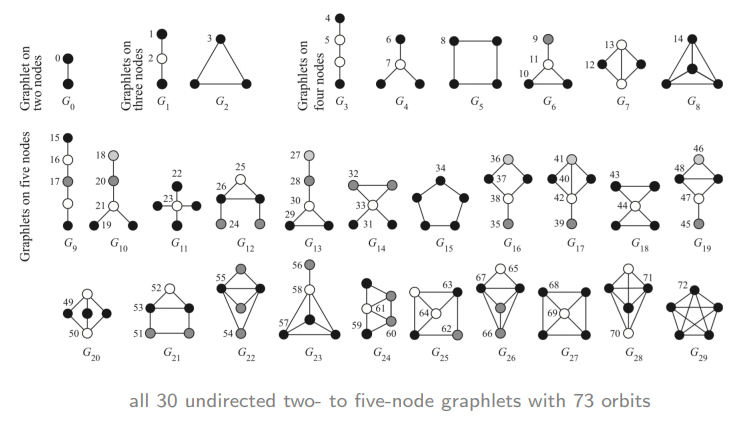
\includegraphics[scale=.5]{graphlets.png}
    \caption{Graphlets and Orbits}
    \label{fig:graphletsAndOrbits}
\end{figure}
\begin{itemize}
    \item \textbf{Fragment:} A connected subgraph.
    \item \textbf{Motifs:} Fragments that occur with a frequency much higher than
        that occuring in a randomly generated graph.
    \item \textbf{Graphlets:} An arbitrary, induced fragment.
An edge is the only two-node graphlet.
    \item \textbf{Induced graphs:} Given a graph $G(V, E)$ and $S \subseteq V$, then $G'(S, E')$
        is a graphlet iff $E' = \{(u, v) | u, v \in V \text{ and } 
        (u, v) \in E \rightarrow (u, v) \in E'\}$
    \item \textbf{Orbits:} Set of all nodes in a graphlet that can be
        swapped with each other while not changing the graph.
\end{itemize}
\subsection*{Concepts}
\begin{itemize}
    \item \textbf{Global vs. local network comparison}:\\
        Global is inappropriate for incomplete networks.

    \item \textbf{Problem of Motifs:}
        They don't take into account infrequent and average subnetworks.

    \item \textbf{GDD: graphlet degree distribution}
\end{itemize}
\section{Literature Review}
\subsection{Hi-C}

Authors of \cite{trieu2015mogen} developed MOGEN.

\subsection{Graphlets}
Graphlet comparison is a novel method used to compare large networks in order to
find local similarities in them.
Authors of \cite{prvzulj2007biological} provide a new measure of PPI
network comparison
based on 73 constraints. This is used in order to compare two large
networks in order to detect similarities.

\cite{milenkoviae2008uncovering} 
 provide heuristics to compare two nodes based on some feature
(or signature) vectors, which is a 73-dimensional vector
$\mathbf{s}^T
= [s_0, s_2, ..., s_{72}]$ where $s_i$ denotes the number of nodes in
the network that are part of an orbit $i$. \\
\textit{Important Result}: Proteins with similar surroundings perform
similar functions.

In \cite{milenkovic2010cancer}, the same author investigates 
cancer-causing genes to find similarities in their signatures. After
clustering the genes based on \textit{signature similarity} criteria,
some clusters contain a lot of cancerous genes.
They use 4 different clustering methods with varying parameters to cluster
the proteins. They then predict the cancer-relatedness of a protein 
$i$ using
an enrichment criteria $\frac{k}{|C_i|}$ where $C_i$ is the cluster
where protein $i$ belongs and $k$ is the number of cancer-causing
proteins in $C_i$ and $|C_i|$ is the size of $C_i$.

Implementations of algorithms of extracting graphlets: \\
\begin{itemize}
    \item GraphCrunch: 
        \url{http://www0.cs.ucl.ac.uk/staff/natasa/graphcrunch2/usage.html}
    \item PGD: \url{http://nesreenahmed.com/graphlets/}
    \item ORCA: Graphlet and orbit counting algorithm \\
        \url{ https://CRAN.R-project.org/package=orca} \\
        This package is in R. In order to install it, type
        \texttt{install.packages("orca")}.
        
\end{itemize}

The authors of \cite{di2010fast} generalized the idea of graphlets to 
ordered graphs were the nodes are labeled in ascending order.
These graphlets are illustrated in Figure \ref{fig:ordered_graphlets}.
As can be viewed, there are a total of 14 orbits for graphlets of size
2 and 3 since the label of graphlets is also included in toplogy.
In the new definition, $d_v^i$ denotes the number of orbit $i$ touches 
node $v$. Each node, is then assigned a vector of length 14 
\footnote{number of orbits in graphlets of size 2 and 3}
$(d_v^1, d_v^2, ..., d_v^{14})$ 
and similarity of two nodes in two contact maps can be compared by
how geometrically close their corresponding vectors are.
\begin{figure}[H]
    \centering
    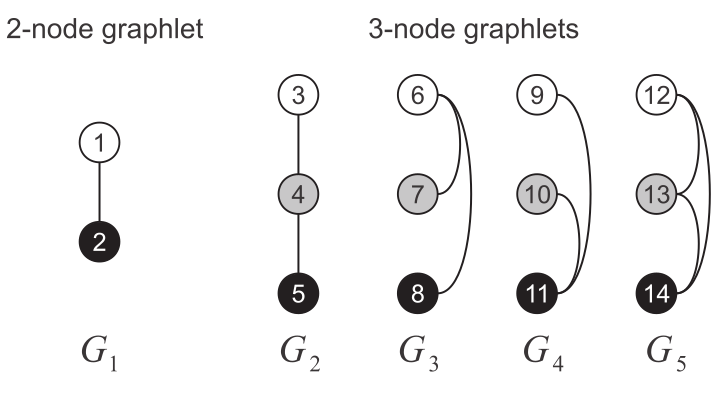
\includegraphics[width=.5\textwidth]{figures/ordered_graphlets.png}
    \caption{The five 2-and 3-node ordered graphlets and the corresponding 14
    automorphism orbits. The ordering of the graphlet nodes within each
    graphlet $G_i,\quad i \in \{1, ... , 5\}$ is represented by their colors: white nodes
    $<$ gray nodes $<$ black nodes}
    \label{fig:ordered_graphlets}
\end{figure}

\subsection{Balanced Network Deconvolution and Residual Networks}
Proposed by \cite{feizi2013network}. They developed a method that
eliminated indirect effect from a weighted graph. Their method
assumes that the observed graph $G_{obs}$ is a summation of its 
direct graph $G_{dir}$ and some indirect terms as follows:
\begin{equation}
    \label{indirect_effects}
    G_{obs} = G_{dir} + G_{dir}^2 + G_{dir} + ...
\end{equation}
They assume also that both $G_{obs}$ and $G_{dir}$ can be 
eigen-decomposed and they have the same eigen-vectors, that is
\begin{equation}
    G_{obs} = X \Sigma_{obs} X^T
\end{equation}
where 
\begin{equation}
    \Sigma_{obs} = 
    \begin{pmatrix}  
        \lambda^{obs}_1 &   0            & \cdots    &    0 \\
        0               &\lambda^{obs}_2 &           &      \\
        \vdots          &                & \ddots    &      \\
        0               &                &           & \lambda^{obs}_n
    \end{pmatrix}
\end{equation}
and
\begin{equation}
    G_{dir} = X \Sigma_{dir} X^T
\end{equation}
where
\begin{equation}
    \Sigma_{dir} = 
    \begin{pmatrix}  
        \lambda^{dir}_1 &   0            & \cdots    &    0 \\
        0               &\lambda^{dir}_2 &           &      \\
        \vdots          &                & \ddots    &      \\
        0               &                &           & \lambda^{dir}_n
    \end{pmatrix}
\end{equation}
so
\begin{equation}
    G_{obs} = X \Sigma_{obs} X^T = X ( \Sigma_{dir} + \Sigma_{dir}^2 + ...) X^T
\end{equation}
They also assume that eigen-values of the direct network are all
between -1 and 1, i.e. 
\begin{equation}
    -1 < \lambda^{dir}_i < 1 \quad \forall 1 \le i \le n
\end{equation}
Thus 
\begin{equation}
    \Sigma_{obs} = \Sigma_{dir} + \Sigma_{dir}^2 + ...
\end{equation}
\begin{equation}
    \lambda_i^{obs} = \sum_{j=1}^{\infty} \lambda^{dir}_{ij} \quad\quad \forall i = 1 ... n
\end{equation}
\begin{equation}
    \lambda_i^{obs} = \frac{\lambda_i^{dir}}{1 - \lambda_i^{dir}}
\end{equation}
\begin{equation}
   \lambda_i^{dir} = \frac{\lambda_i^{obs}}{1 + \lambda_i^{obs}} 
\end{equation}

\textbf{Source codes:} 
\begin{itemize}
    \item Python: \url{https://github.com/gidonro/Network-Deconvolution} 
    \item Matlab: \url{http://compbio.mit.edu/nd/}
\end{itemize}

Authors of \cite{sun2015improving} proposed ...
\subsection{Weighted graph comparison}
\url{https://www.cs.cmu.edu/~jingx/docs/DBreport.pdf}

\url{https://en.wikipedia.org/wiki/Gromov%E2%80%93Hausdorff_convergence}

Authors of \cite{soufiani2012graphlet} propose a graphlet
decomposition method
which considers situations where we observe an undirected
weighted network, encoded by a symmetric adjacency matrix with integer entries and diagonal
elements equal to zero. The term graphlet here is UNRELATED to the
Przulj graphlet.

Authors of \cite{ginestet2011statistical} developed Statistical Network (SPN) analysis
where the choice of thresholding value is made by statistical inference.
This method works within the framework of design of experiments where the same
network can be extracted for different individuals under different treatments. The
effect of those treatments can then be infered using this method.
In \cite{ginestet2011statistical} for example, they studied neuron connectivity
networks among 43 subjects for 4 different memory tasks (0-back, 1-back, 2-back and
3-back), and obtained the following thresholded networks. The results of which can 
be viewed in Figure \ref{fig:thresholded_adjacency}.

Their method can be very usefull if a large population of information from the same
chromosomes exist.
\begin{figure}
    \centering
    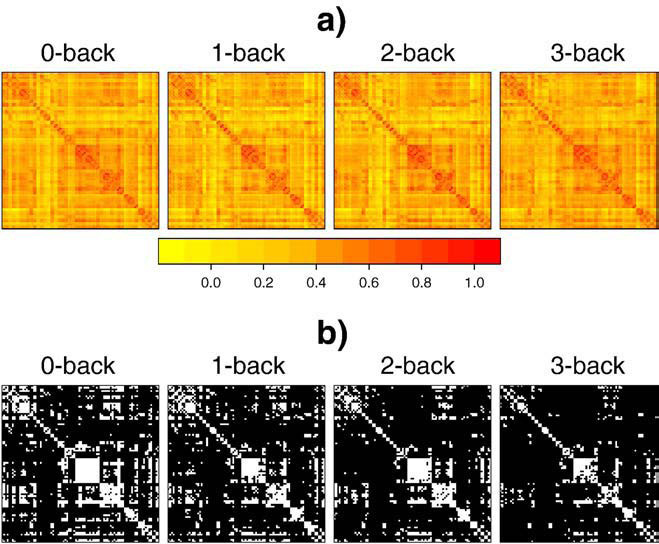
\includegraphics[width=.5\textwidth]{figures/thresholded_adjacency.png}
    \caption{}
    \label{fig:thresholded_adjacency}
\end{figure}

Distance between two weighted graphs can be measured based on \cite{daneshpajouh2009metric}:\\
$d(G_1, G_2) = |\displaystyle\sum_{w\in V_1} w -
\displaystyle\sum_{v \in V_2} v|$

Exhaustive enumeration of all graphlets being
prohibitively expensive, \cite{shervashidze2009efficient} introduce two
theoretically grounded speedup schemes, one
based on sampling and the second one specifically
designed for bounded degree graphs

\section{Problems and Questions}
\begin{enumerate}
    \item Can we convert larger Hi-C data sets by combining data from 
        several loci? This way we can create a DOE of different 
        individuals.
    \item How can we verify our results? Do we have any information on 
        similarities that we already know exist?
    \item how do we get inter-chromosomal graphs?
        I was not able to find them.
    \item Is there indirect depencecies in the Hi-graphs? How are they caused?
    \item How to run the algorithms on such huge matrices?
    \item What are random graph models?
    \item As far as I get, graphlet distribution is a means of finding similarities
        in graphs. What we are trying to do is to find dissimilarities. is it 
        the right track to go?
\end{enumerate}

\section{Experiments and Observations}
I have changed the network deconvolution code where it deals
with scaling factor. The rationale behind it was not clear to me
so I replaced it with my own understanding of it which might not 
be correct.

The intensity values in each data set follows an exponential
distribution, that is the majority of the intensities lie
close to the minimum value while some intensities are absurdly
large.
Because of this, thresholding intensity values based on quantiles (percentiles)
cannot be helpful since first and third quartiles are very close to each other
but very far from the maximum value.
\begin{figure}[H]
    \centering
    \begin{subfigure}[b]{.45\textwidth} 
        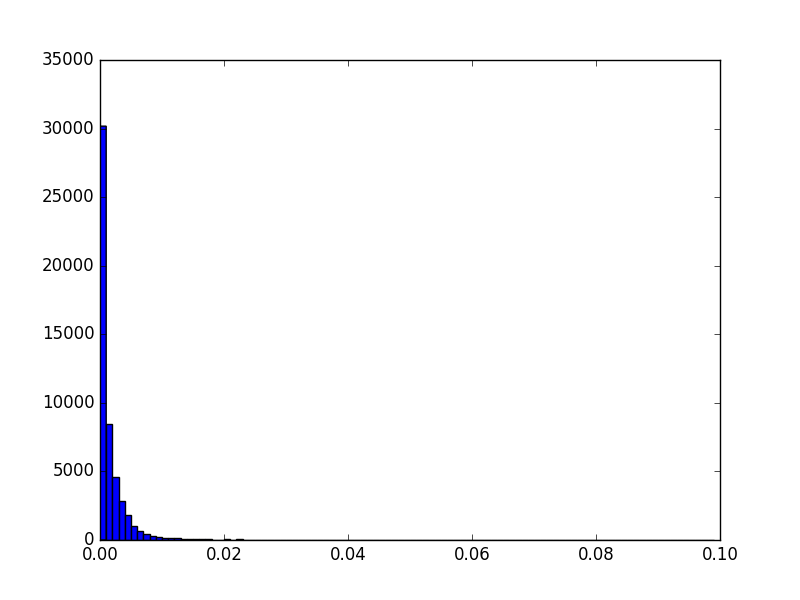
\includegraphics[width=\textwidth]{figures/hist01.png}
        \caption{}
        \label{fig:hist01}
    \end{subfigure}
    \begin{subfigure}[b]{.45\textwidth}
        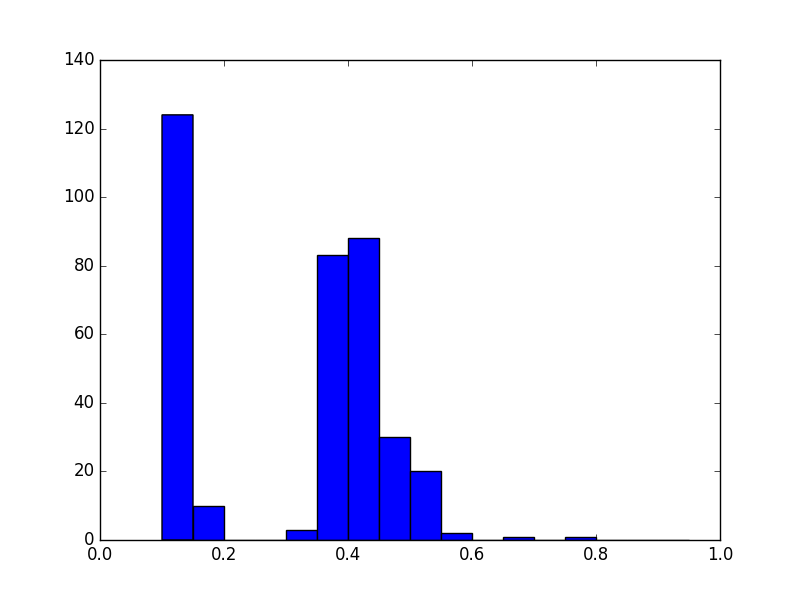
\includegraphics[width=\textwidth]{figures/hist02.png}
        \caption{}
        \label{fig:hist02}
    \end{subfigure}
    \caption{\ref{fig:hist01} is a histogram of intensities form 
    ``\texttt{chr1\_1mb\_matrix}'',
    in the interval of $[0, 0.1]$ and bin size of $0.005$.
    \ref{fig:hist02} is a histogram of the same data
    but for interval of $[0.1, 1]$ and bin size of $0.01$.
    As can be seen, the two histograms are orders of magnitude
    different in terms of frequency.}
    \label{fig:hists}
\end{figure}
Each row and column in the graphs represents a loci on the chromosome,
the next row (column) represents the adjacent loci on the same chromosome,
thus the graph cannot be scrambled, that is, it is constructed as a stack
of interaction intensities of a locus with all other loci on the chromosome.
You cannot just swap two rows in the graph and have the same information since
the order is important. The only valid case is when last rows are removed 
and stacked on top of the graph.

Taking a logarithm can be very useful in this case. As can be viewed in Figures
\ref{fig:all_hists01} and \ref{fig:all_hists_deconvoluted01}, you can see that the data for 
all chromosomes look normal.
\begin{landscape}
\begin{figure}[H]
    \centering
    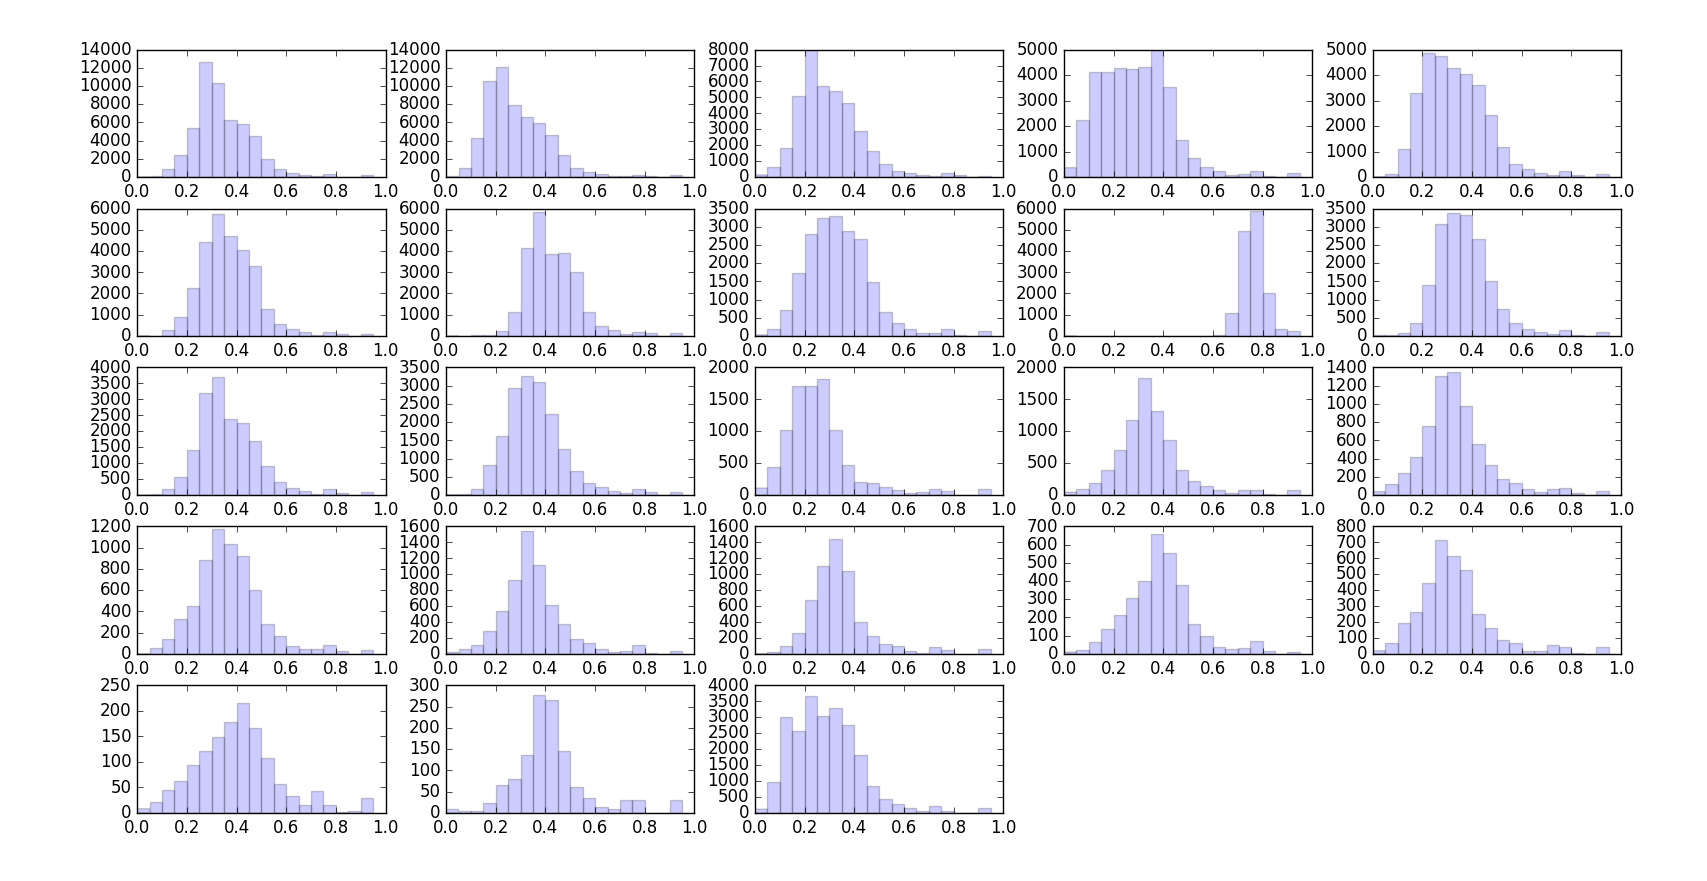
\includegraphics[width=1.5\textwidth]{figures/all_hists01.png}
    \caption{The histogram of the logarithm of the data for all 23
            chromosomes. The data looks normal now.}
    \label{fig:all_hists01}
\end{figure}

\begin{figure}[H]
    \centering
    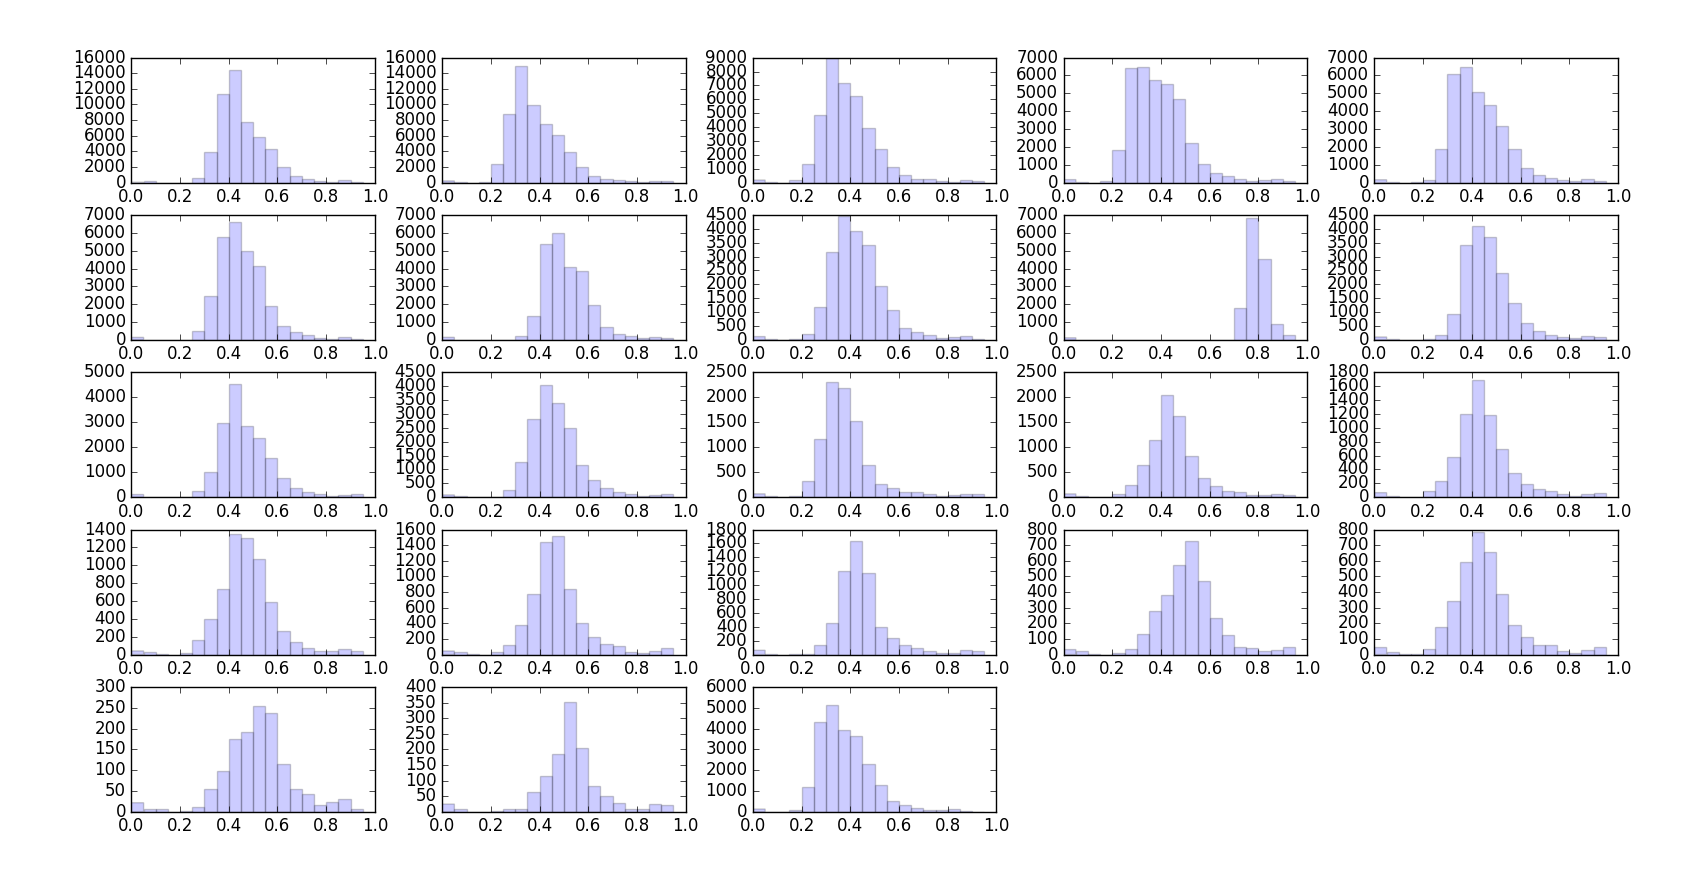
\includegraphics[width=1.5\textwidth]{figures/all_hists_deconvoluted01.png}
    \caption{The histogram of the deconvoluted  data in Figure 
            \ref{fig:all_hists01}. }
    \label{fig:all_hists_deconvoluted01}
\end{figure}
\end{landscape}

We decided to lock our data set on \href{http://sysbio.rnet.missouri.edu/bdm_download}{this}
dataset, since it includes Hi-C data for both normal test cells and 3 various cancerous
cells. This allows for the sort of comparison we are looking for in this study.

Cleaning the data requires some step that I'm not familiar yet. For example a normalized
Hi-C heatmap for chromosome 1 should look like something like \ref{fig:normalized_heatmap},
which can be found 
\href{http://sysbio.rnet.missouri.edu/T0510/tmp_download/link_to_download_genome_data/}{here},
but what I have managed to get from raw data is \ref{fig:my_result}, which clearly is
not normalized.
\begin{figure}[H]
    \centering
        \begin{subfigure}[b]{.4\textwidth}
            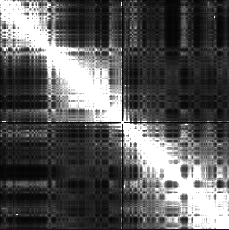
\includegraphics[width=\textwidth]{figures/normalized_heatmap.png}
            \caption{}
            \label{fig:normalized_heatmap}
        \end{subfigure}
        \begin{subfigure}[b]{.4\textwidth}
            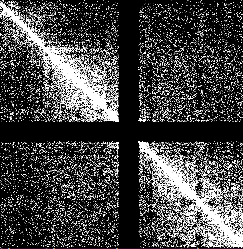
\includegraphics[width=\textwidth]{figures/my_result.png}
            \caption{}
            \label{fig:my_result}
        \end{subfigure}
    \caption{As can be seen, \ref{fig:my_result} is not
                as smooth as \ref{fig:normalized_heatmap}.
                The black area in \ref{fig:my_result} account for 
                19 rows and columns, which is
                exactly the difference between the number of columns 
                in \ref{fig:my_result} and \ref{fig:normalized_heatmap}.
                }
    \label{fig:heatmap_comparison}
\end{figure}

Based on \cite{wang2013properties}, two normalization methods can be 
implemented on a contact matrix. The first of is Sequential Component 
Normalization (SCN \cite{cournac2012normalization})
and the other is simple Pearson's correlation. 

In SCN, each column of the contact matrix is divied by its norm, then
its rows are divided by theirs norms. This process continues until the 
contact matrix is symmetric again.

In Pearson's correlation, a matrix $C$ is produced where $C_{ij}$
is the pearson correlation of rows i and j. 

I have come up with what I call the \textit{pyramid algorithm}
where I simply apply a pyramid down and then pyramic up
on contact matrices to fill the empty spaces between. 
This algorithm is readily available
in OpenCV \footnote{www.opencv.org}.

The results of the normalizations on chrmosome 1 of a normal
cell is presented in Figure \ref{fig:normalizations}.

\begin{figure}[H]
    \centering
    \begin{subfigure}[b]{.3\textwidth}
        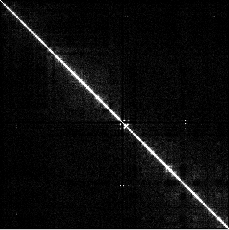
\includegraphics[width=\textwidth]{figures/original_cleaned.png}
        \caption{}
        \label{fig:original_cleaned}
    \end{subfigure}
    \begin{subfigure}[b]{.3\textwidth}
        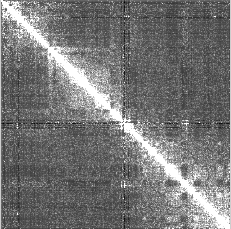
\includegraphics[width=\textwidth]{figures/pearson.png}
        \caption{}
        \label{fig:pearson}
    \end{subfigure}
    \begin{subfigure}[b]{.3\textwidth}
        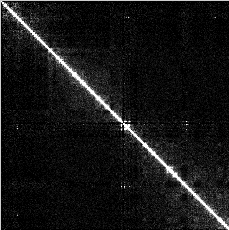
\includegraphics[width=\textwidth]{figures/scn.png}
        \caption{}
        \label{fig:scn}
    \end{subfigure}
    \begin{subfigure}[b]{.3\textwidth}
        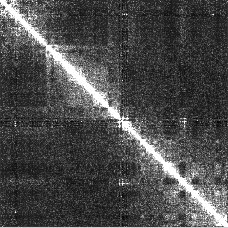
\includegraphics[width=\textwidth]{figures/scn+pearson.png}
        \caption{}
        \label{fig:scn+pearson}
    \end{subfigure}
    \begin{subfigure}[b]{.3\textwidth}
        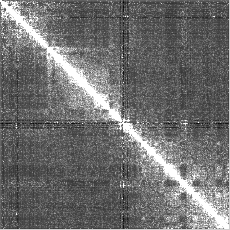
\includegraphics[width=\textwidth]{figures/pearson+scn.png}
        \caption{}
        \label{fig:pearson+scn}
    \end{subfigure}
    \begin{subfigure}[b]{.3\textwidth}
        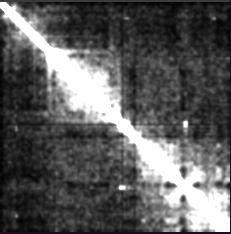
\includegraphics[width=\textwidth]{figures/pyr.png}
        \caption{}
        \label{fig:pyr}
    \end{subfigure}
\caption{Results of different normalizing methods: 
    \ref{fig:original_cleaned} is the original matrix of \ref{fig:my_result}
    with the 19 empty rows and columns removed.
    \ref{fig:pearson} demonstrates the result of applying pearson normalization
    to the \ref{fig:original_cleaned}.
    In the same manner \ref{fig:scn} demonstrates the 
    result of applying scn to \ref{fig:original_cleaned}.
    \ref{fig:scn+pearson} shows the result of applying pearson to 
    \ref{fig:scn} and \ref{fig:pearson+scn} illustrates
    result of applying scn to \ref{fig:pearson}.
    \ref{fig:pyr} is the result of applying my pyramid method to the image
    which makes it somehow smooth and as I will describe later, will
    significantly improve histogram of logarithm matrix.
    }
    \label{fig:normalizations}
\end{figure}

Figure \ref{fig:pearson_hist} illustrates the result of histograms of
logarithms of figures that result from pearson normalization or chromosomes
1 through 22 and chromosome X (the last one).

Figure \ref{fig:pyr_hist_1mb} illustrates the result of histograms of
logarithms of figures that result from applying pyramid normalization
on the contact matrices of chromosomes
1 through 22 and chromosome X (the last one).
\begin{landscape}
    \begin{figure}[H]
        \centering
        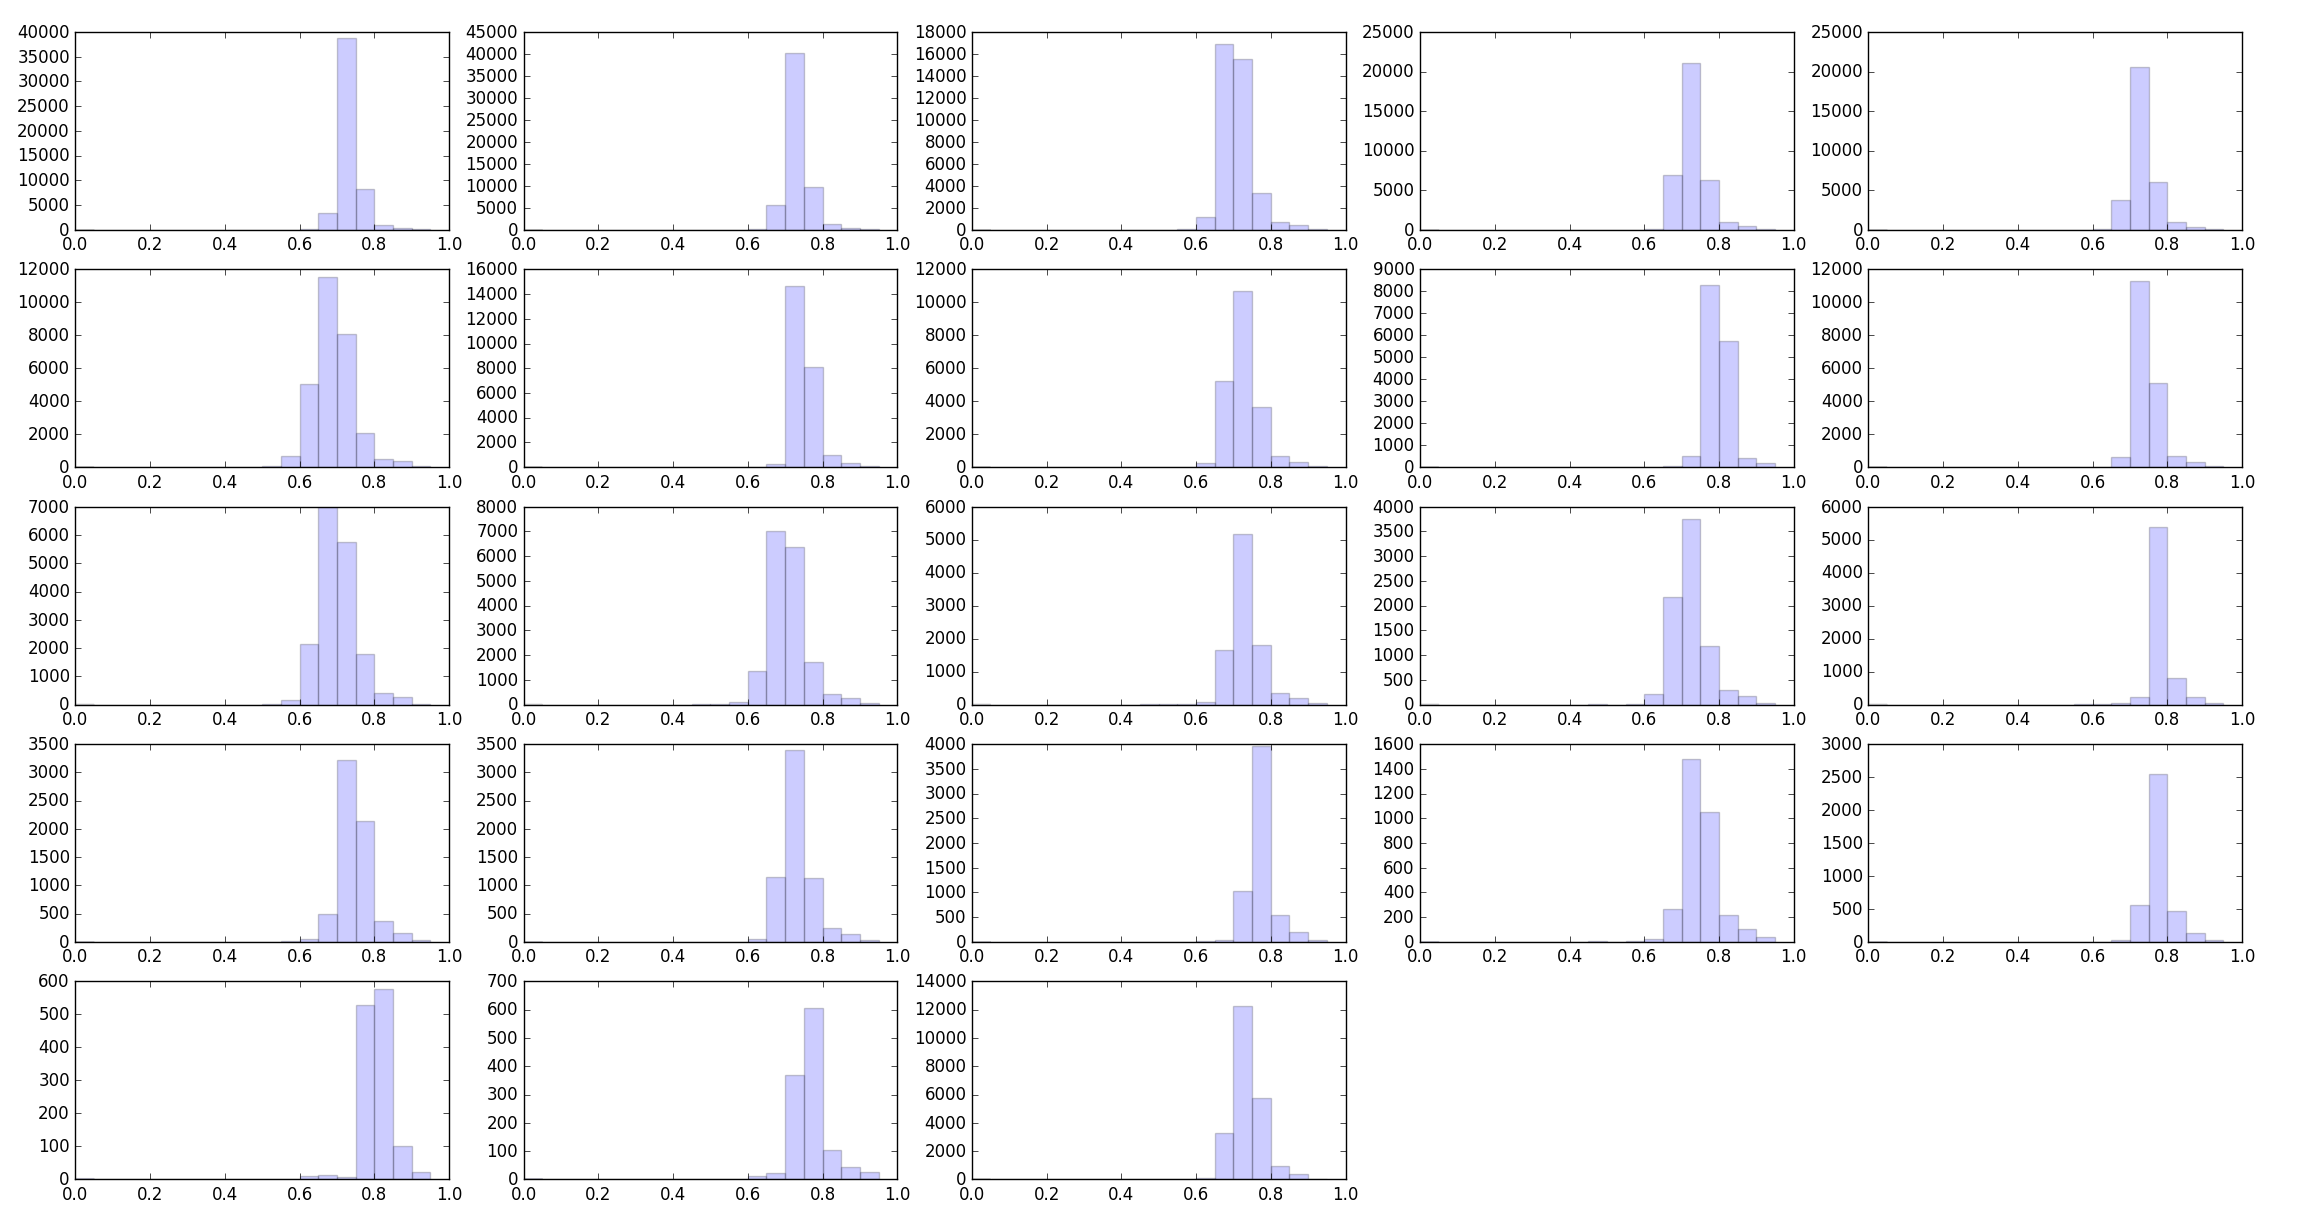
\includegraphics[width=1.5\textwidth]{figures/pearson_hist.png}
        \caption{}
        \label{fig:pearson_hist}
    \end{figure}

\begin{figure}[H]
    \centering
    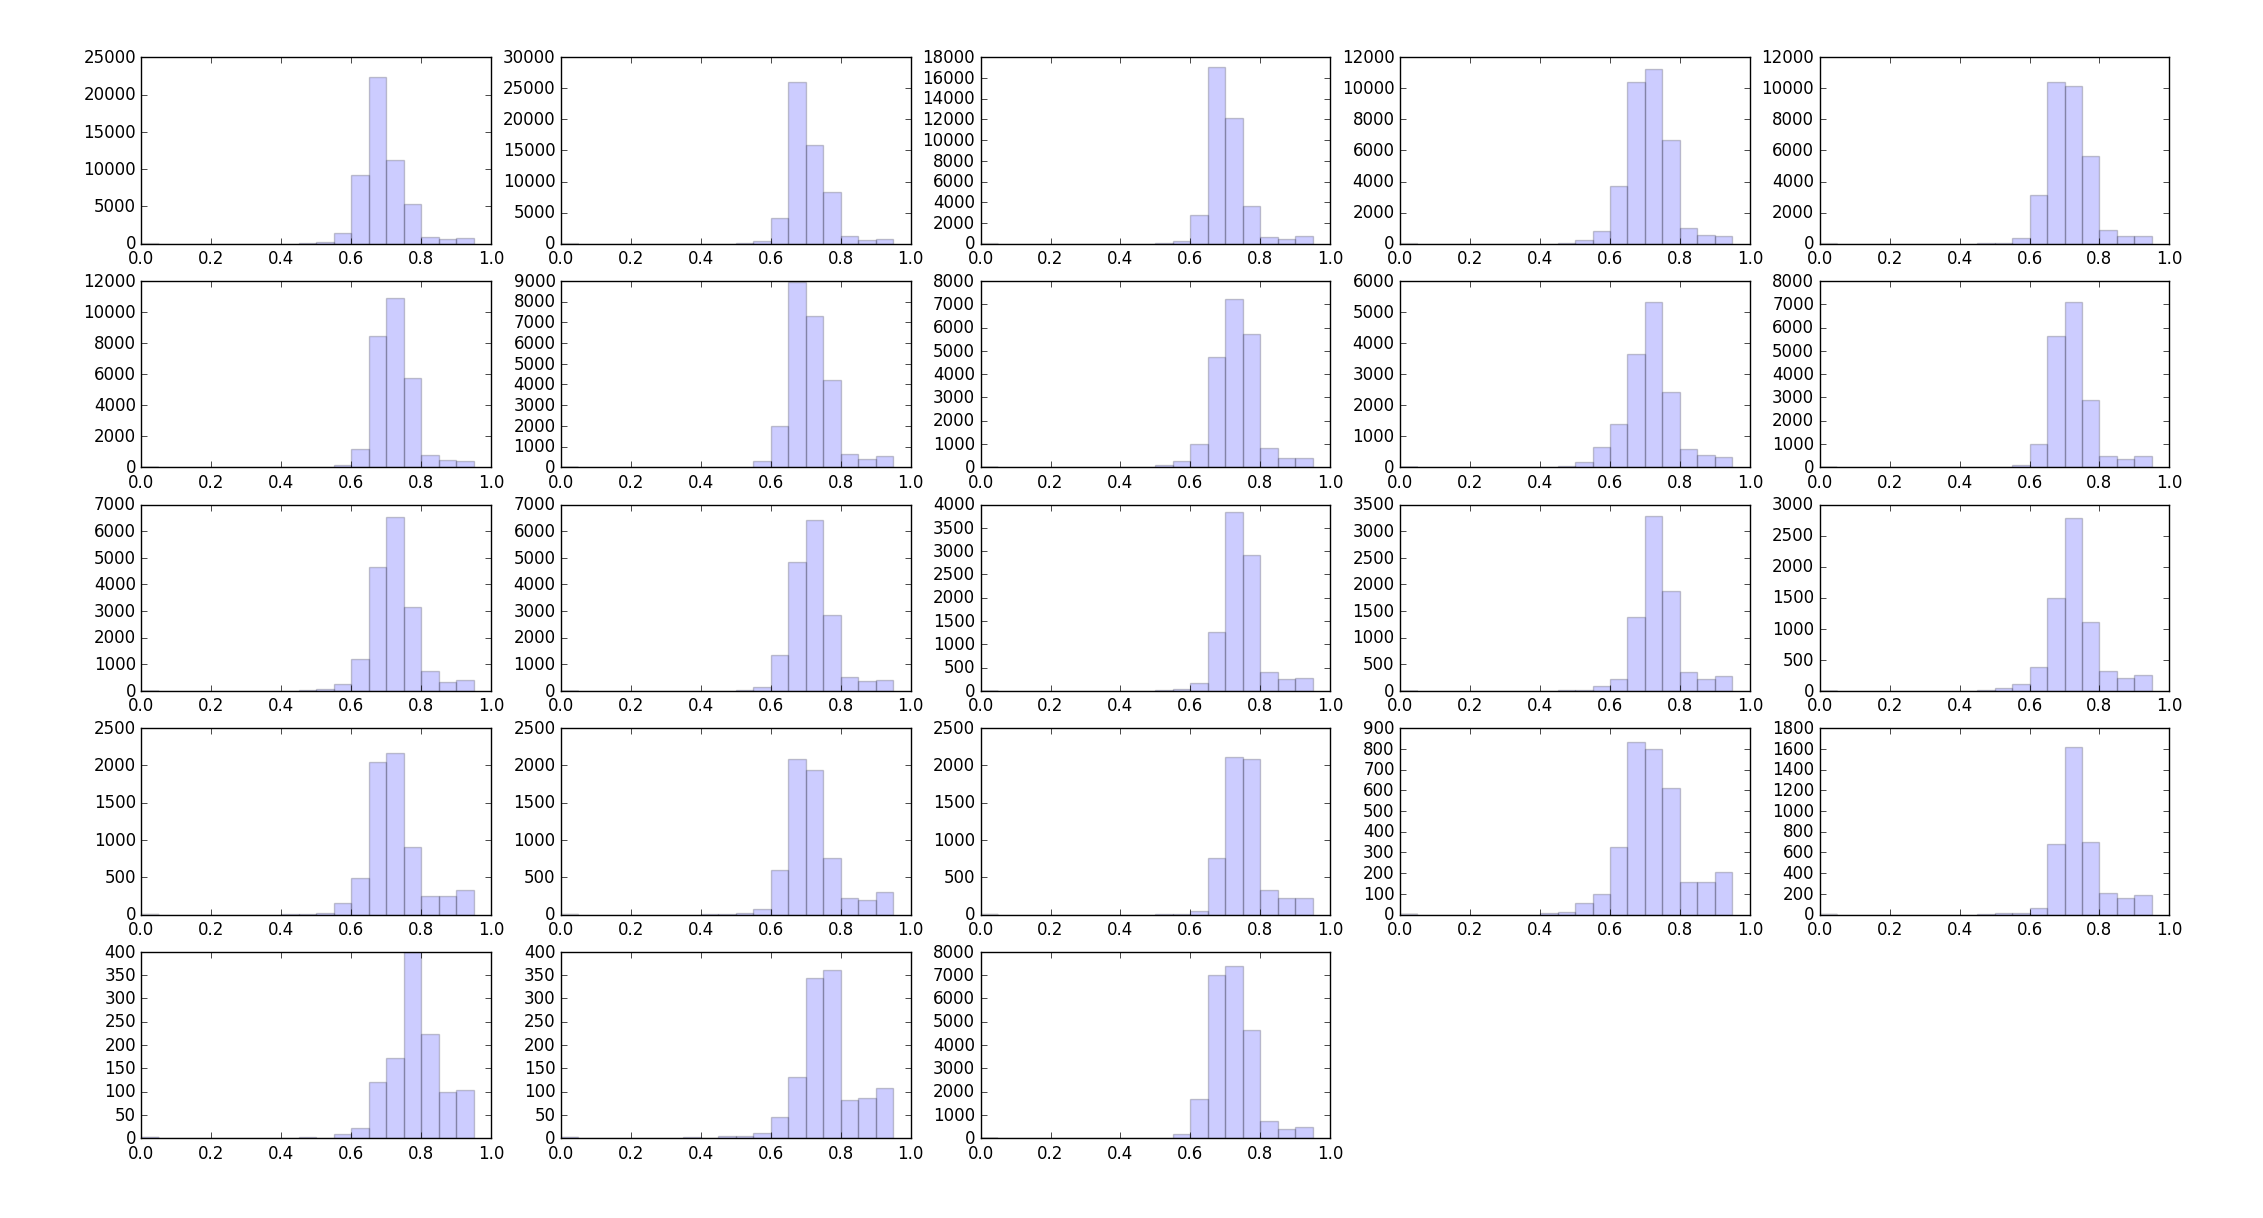
\includegraphics[width=1.5\textwidth]{figures/pyr_hist_1mb.png}
    \caption{}
    \label{fig:pyr_hist_1mb}
\end{figure}
\end{landscape}

\subsection*{ALL and MIT cell comparison}
One idea is the vary the threshold limits on the two indices to 
find the optimal set of thresholds $(t_{ALL}, t_{MIT})$, where 
the difference between the two pixels are minimum. The remaining
pixels that are still different are the ones that are definitely
correct. In this case, the objective function should be properly
penalized in order to prevent the thresholds from getting too
high or too low.
\begin{figure}[H]
    \centering
    \begin{subfigure}[b]{.45\textwidth} 
        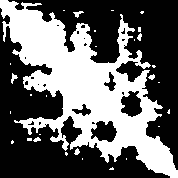
\includegraphics[width=\textwidth]{figures/ALL_60per_thresh.png}
        \caption{}
        \label{fig:all_thresh}
    \end{subfigure}
    \begin{subfigure}[b]{.45\textwidth}
        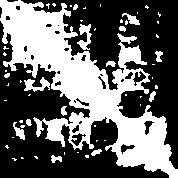
\includegraphics[width=\textwidth]{figures/MIT_60per_thresh.png}
        \caption{}
        \label{fig:mit_thresh}
    \end{subfigure}
    \begin{subfigure}[b]{.45\textwidth}
        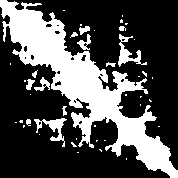
\includegraphics[width=\textwidth]{figures/ALL_MIT_common.png}
        \caption{}
        \label{fig:all_mit_common}
    \end{subfigure}
    \begin{subfigure}[b]{.45\textwidth}
        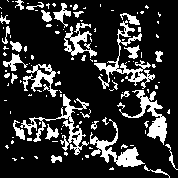
\includegraphics[width=\textwidth]{figures/ALL_MIT_diff.png}
        \caption{}
        \label{fig:all_mit_diff}
    \end{subfigure}
    \caption{\ref{fig:all_thresh} is HiC contact matrix of 
             chromosome 14 of ALL cell and
             \ref{fig:mit_thresh} is the contact matrix of
             the same chromosome in MIT cells. 
             Both matrices are thresholded based on their 60th
             percentile. \ref{fig:all_mit_common} is the common pixels
             and \ref{fig:all_mit_diff} is the pixels where they 
             are different.}
\end{figure}
%\input{../scripts/logs/2018-01-31.log}
\section{Resources}
\textbf{Publications related to Hi-C:}
\begin{enumerate}
    \item \url{https://www.ncbi.nlm.nih.gov/pmc/articles/PMC2858594/}
    \item \url{http://journals.plos.org/plosone/article?id=10.1371/journal.pone.0058793 }
    \item \url{http://nar.oxfordjournals.org/content/42/7/e52.full}
    \item \url{http://bioinformatics.oxfordjournals.org/content/early/2015/12/31/bioinformatics.btv754.abstract?keytype=ref&ijkey=A97WhKqBiEIcuzd}
    \item \url{https://www.ncbi.nlm.nih.gov/pmc/articles/PMC4417147/}
    \item \url{http://www.pnas.org/content/112/47/E6456.full}
    \item \url{http://www.pnas.org/content/113/12/E1663.full}
\end{enumerate}
\textbf{Hi-C Datasets:}
\begin{enumerate}
    \item Original Datasets: \url{https://bcm.app.box.com/v/aidenlab/folder/11234760671}
    \item Including cancerous cells: \url{http://sysbio.rnet.missouri.edu/T0510/tmp_download/link_to_download_genome_data/}
    \item Chromosome3D project: \url{http://sysbio.rnet.missouri.edu/bdm_download/chromosome3d/}
\end{enumerate}
\textbf{Contact Matrix Analysis:}
\begin{enumerate}
    \item \url{https://omictools.com/contact-matrix-normalization-category}
    \item \url{http://hifive.docs.taylorlab.org/en/latest/}
\end{enumerate}

\textbf{Labs working on 3D Human Genome:}

\begin{enumerate}
    \item \url{http://mirnylab.mit.edu}
    \item \url{http://dostielab.biochem.mcgill.ca}
    \item \url{http://www.aidenlab.org/}
    \item \url{http://web.cmb.usc.edu/people/alber/index.htm}
    \item \url{http://calla.rnet.missouri.edu/cheng/nsf_career.html}
\end{enumerate}
\textbf{Resources related to Graphlet:}

\begin{enumerate}
    \item \url{https://en.wikipedia.org/wiki/Graphlets}
    \item \url{https://academic.oup.com/bioinformatics/article/23/2/e177/202080/Biological-network-comparison-using-graphlet}
    \item \url{http://www0.cs.ucl.ac.uk/staff/N.Przulj/index.html}
\end{enumerate}

\bibliography{lit}
\bibliographystyle{unsrt}
\end{document}
